
\documentclass[]{article}
\usepackage{graphicx}
\usepackage{amsmath}

\usepackage{subcaption}
\usepackage{color}
\usepackage{algorithm}
\usepackage{listings}
\usepackage[pagebackref,breaklinks,colorlinks]{hyperref}
\usepackage{cleveref}
%opening
\title{Report for Computer GraphicII, HW2 \\ 2D Skeleton extraction by Chordal Axis Transform (CAT) }
\author{Sixun Dong, 2021233155}


\begin{document}

\maketitle
Acknowledgements:

Deadline: 2022-03-31 23:59:59


You should answer the questions in \textbf{English}


You can choose C++ or Python, and no restrictions on programming framework. You can freely use frameworks such as openGL.

The \textbf{report} submits as a PDF file to gradscope, the programming part should package all the files include code, input files, executable file, readme.txt, and report. The \textbf{package} name is  \textbf{your\_student\_name+student\_id.zip}.

You will get Zero if the code not passing the plagiarism check.
\newpage
\section{2D Skeleton extraction by CAT}
\subsection{Delaunay Triangulation (40 points)}
Implement 2D Delaunay Triangulation for any given sampling points. You are required to provide at least five examples (sample on the contours of some 2D shapes) and corresponding DT visualization. 

\paragraph{\color{red}Solution:}

The algorithm is from the paper\footnote[1]{\url{http://paulbourke.net/papers/triangulate/}} and refer to the note\footnote[2]{\url{https://www.jianshu.com/p/172749e6116a}}. Pseudo code is as \cref{fig:q1code} shown.
\begin{figure}[ht]
    \centering
    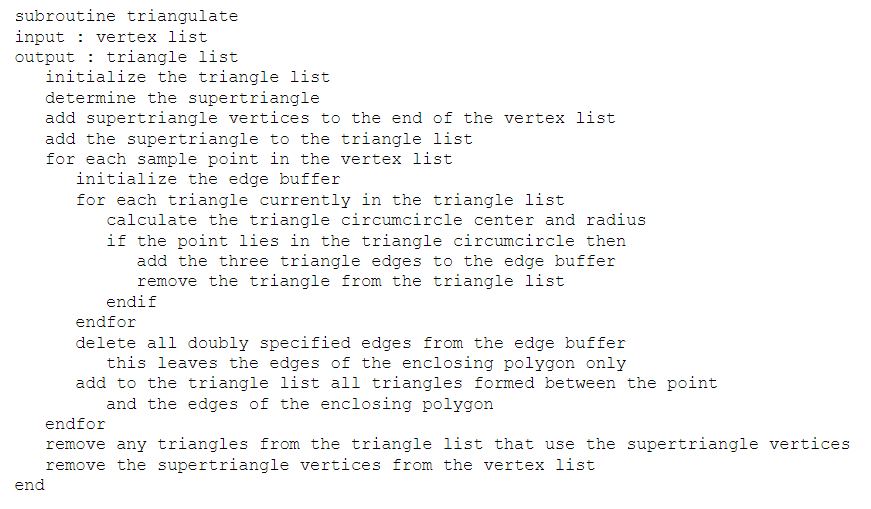
\includegraphics[width=\textwidth]{q1code.png}
    \caption{The pseudo code of DT, which is from the paper$^1$.}
    \label{fig:q1code}
\end{figure}


The result as \cref{fig:q1} shown, it contains five examples \cref{fig:8,fig:10,fig:12,fig:20,fig:50}, which are generated by DT with different numbers of random points.

\begin{figure}[ht]
    \centering
    \begin{subfigure}{0.30\textwidth}
        \centering
        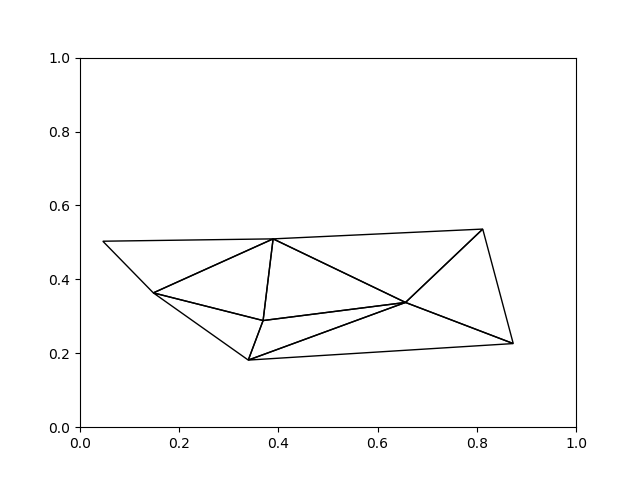
\includegraphics[width=1\linewidth]{8p.png}
        \caption{DT with 8 random points.}
        \label{fig:8}
    \end{subfigure}
    \hfill  % 这个\hfill指令为插入弹性长度的空白,看情况选择加不加。
    \begin{subfigure}{0.30\textwidth}
        \centering
        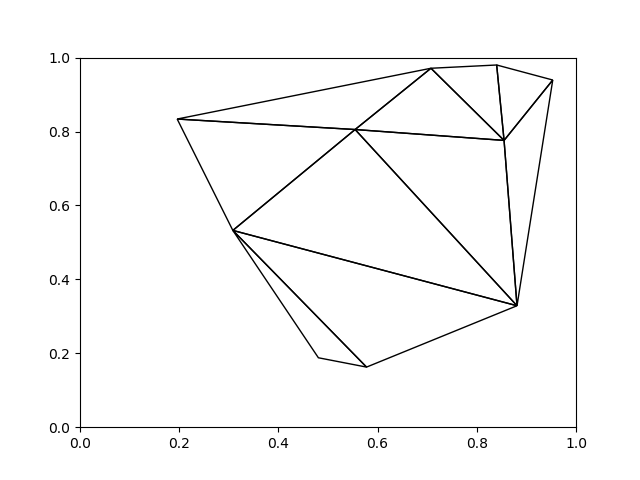
\includegraphics[width=\linewidth]{10p.png}
        \caption{DT with 10 random points.}
        \label{fig:10}
    \end{subfigure}
    \hfill
    \begin{subfigure}{0.30\textwidth}
        \centering
        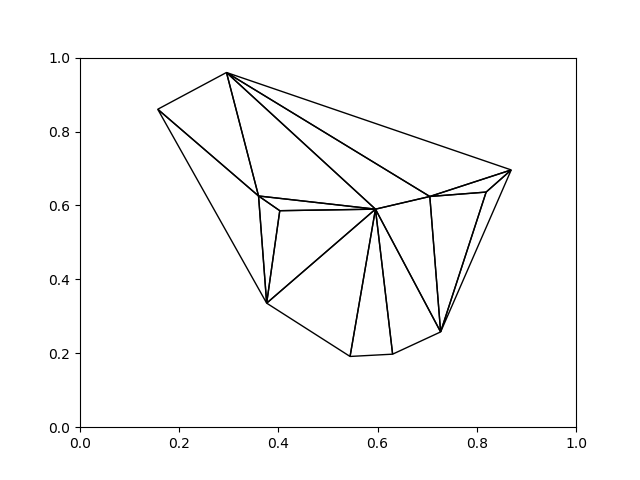
\includegraphics[width=\linewidth]{12p.png}
        \caption{DT with 12 random points.}
        \label{fig:12}
    \end{subfigure}    
    \hfill
    \begin{subfigure}{0.30\textwidth}
        \centering
        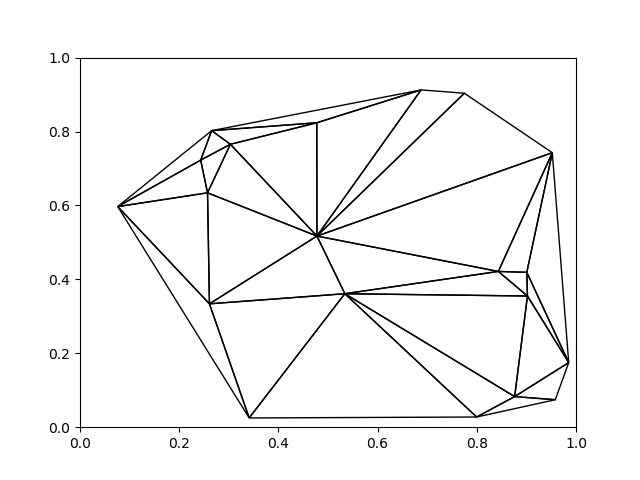
\includegraphics[width=\linewidth]{20p.png}
        \caption{DT with 20 random points.}
        \label{fig:20}
    \end{subfigure}
    \quad
    \begin{subfigure}{0.30\textwidth}
        \centering
        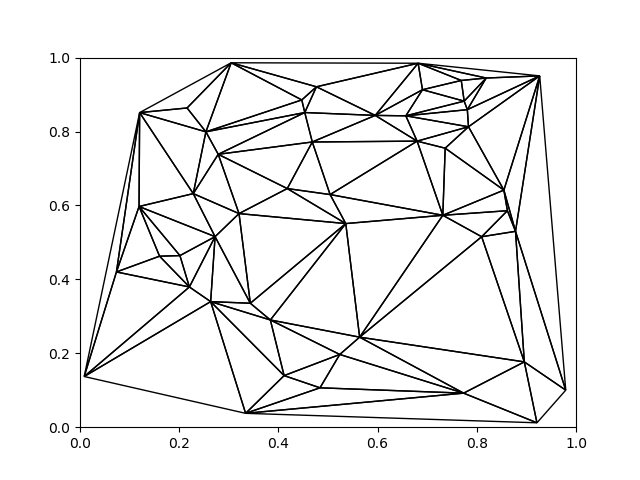
\includegraphics[width=\linewidth]{50p.png}
        \caption{DT with 50 random points.}
        \label{fig:50}
    \end{subfigure}
    
    \caption{
        Five examples of DT.
    }
    \label{fig:q1}
\end{figure}




\newpage
\newpage
\subsection{CAT (30 points)}
Implement CAT and visualize the skeleton results of the above examples. 

\paragraph{\color{red}Solution:}

The implementation uses \textit{Triangle}\footnote[3]{\url{https://rufat.be/triangle/}} module to help generating input data, implementing CDT algorithm and visualization.

The implementation have four step.
\begin{itemize}
    \item[(1)] Use \textit{Triangle} to generate the input data which is a face.
    \item[(2)] Use \textit{Triangle.triangulate()} to generate CDT.  
    \item[(3)] Traverse\footnote[4]{The algorithm refers to the $10^{th}$ page of the paper: \url{https://citeseerx.ist.psu.edu/viewdoc/download?doi=10.1.1.57.3204&rep=rep1&type=pdf}} the triangles and divide them into three kinds. They independently have one , two, or three edges on the boundary.
    \item[(4)] Use the CAT algorithm in the $3^{rd}$ slide to connect the middle points of the edges.
\end{itemize}
\begin{figure}[ht]
    \centering
    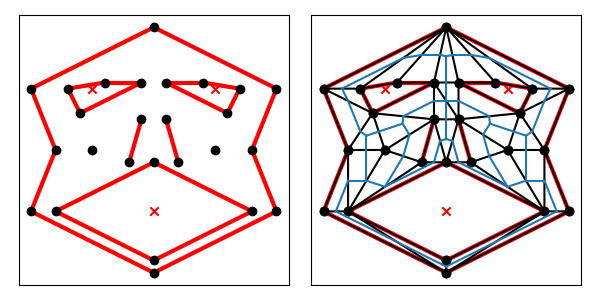
\includegraphics[width=\textwidth]{q2.png}
    \caption{The result of Q2.}
    \label{fig:q2}
\end{figure}


\newpage
\subsection{Comparison (30 points)}
Compare and analyze the skeleton generated by CAT and by the connected centers of circumcircles of DT triangles on different sampling densities on the contours of 2D shapes. 


\paragraph{\color{red}Solution:} 
By using \textit{Triangle} to generate different numbers of triangles.
The result as \cref{fig:q3cdt,fig:q3dt} shown, by limiting the minimum angle of triangles, we could abtain the different numbers of triangles. And the result figure out that more triangles do not necessarily lead to the best results. CAT can achieve better results with the least number of triangles.

\begin{figure}[ht]
    \centering
    \begin{subfigure}{0.30\textwidth}
        \centering
        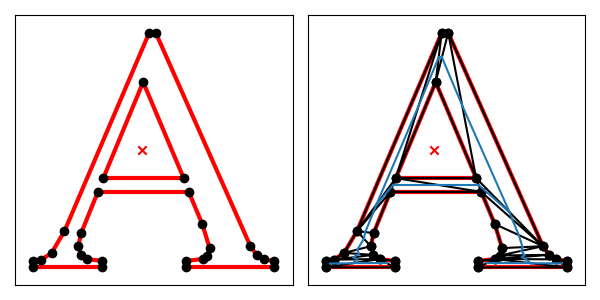
\includegraphics[width=1\linewidth]{cdt1_29.png}
        \caption{The result of CDT with 29 triangles and the minimum angle of triangles is 0.}
        \label{fig:cdt1}
    \end{subfigure}
    \hfill  % 这个\hfill指令为插入弹性长度的空白,看情况选择加不加。
    \begin{subfigure}{0.30\textwidth}
        \centering
        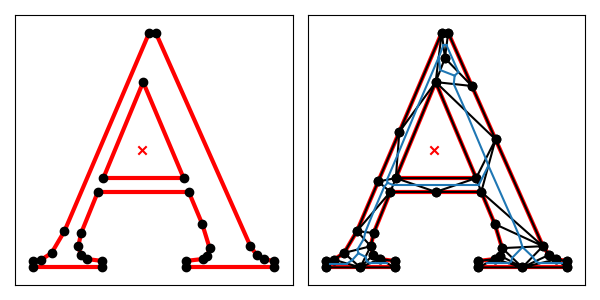
\includegraphics[width=\linewidth]{cdt2_43.png}
        \caption{The result of CDT with 43 triangles and the minimum angle of triangles is 10.}
        \label{fig:cdt2}
    \end{subfigure}
    \hfill  % 这个\hfill指令为插入弹性长度的空白,看情况选择加不加。
    \begin{subfigure}{0.30\textwidth}
        \centering
        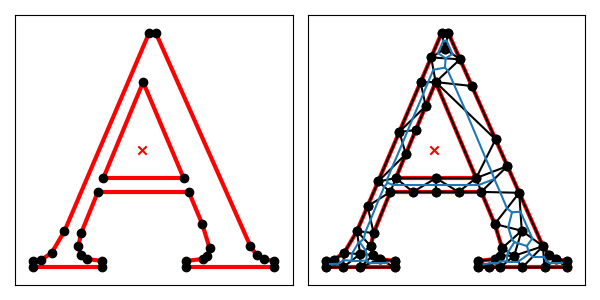
\includegraphics[width=\linewidth]{cdt3_77.png}
        \caption{The result of CDT with 77 triangles and the minimum angle of triangles is 20.}
        \label{fig:cdt3}
    \end{subfigure}
    \caption{
        CAT: The different numbers of triangles by limiting the minimum angle of triangles.
    }
    \label{fig:q3cdt}
\end{figure}

\begin{figure}[ht]
    \centering
    \begin{subfigure}{0.30\textwidth}
        \centering
        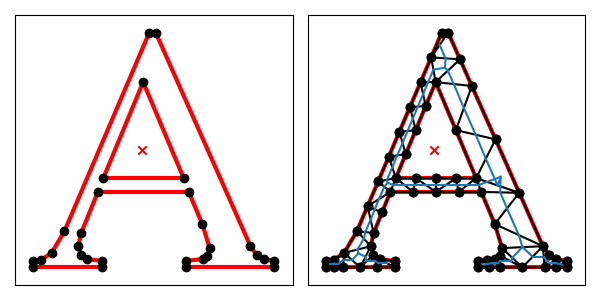
\includegraphics[width=1\linewidth]{dt1_66.png}
        \caption{The result of DT with 66 triangles and the minimum angle of triangles is 0.}
        \label{fig:dt1}
    \end{subfigure}
    \hfill  % 这个\hfill指令为插入弹性长度的空白,看情况选择加不加。
    \begin{subfigure}{0.30\textwidth}
        \centering
        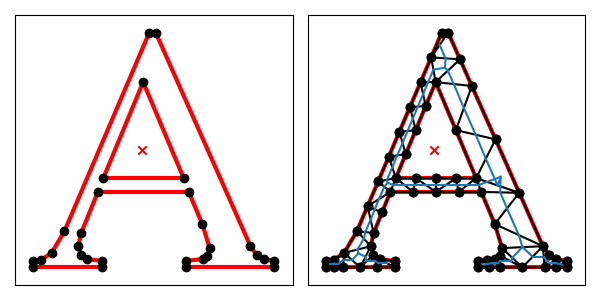
\includegraphics[width=\linewidth]{dt2_66.png}
        \caption{The result of DT with 66 triangles and the minimum angle of triangles is 10.}
        \label{fig:dt2}
    \end{subfigure}
    \hfill  % 这个\hfill指令为插入弹性长度的空白,看情况选择加不加。
    \begin{subfigure}{0.30\textwidth}
        \centering
        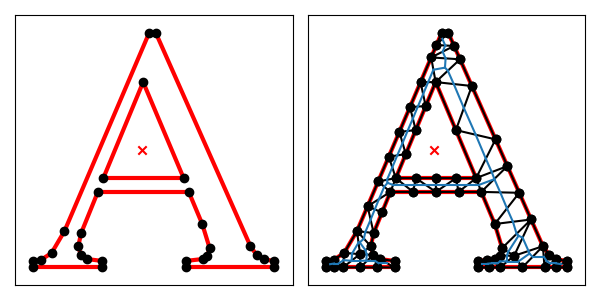
\includegraphics[width=\linewidth]{dt3_82.png}
        \caption{The result of DT with 82 triangles and the minimum angle of triangles is 20.}
        \label{fig:dt3}
    \end{subfigure}
    \caption{
        DT: The different numbers of triangles by limiting the minimum angle of triangles.
    }
    \label{fig:q3dt}
\end{figure}

\end{document}
